\section{Scaling laws}


Metal organic framework(MOF): porus materials. Able to store substance (e.g. Water) at low temperature and release when heated.

Void volume (porosity) is defined as
\[
\epsilon = \frac{V_pores}{V_materials}
\]
\begin{itemize}
    \item Micropores (<2nm)
    \item Mesopores (2-50nm)
    \item Macropores (>50nm)
\end{itemize}
\subsection{Surface Tension and surface energy}
Water runner on water, leg sinks \(\rightarrow\) Energy is stored in surface energy:
\[
E_s = \gamma \cdot A
\]
\(\gamma\): specific surface energy/surface tension \(\text{J/m}^2\) or \(\text{N/m}^2\) 

The surface tension tries to keep the surface of a fluid as small as possibel \(\rightarrow\) Drops of liquid are spherical.

\section{Condensed matter}
Type of bonds:
\begin{itemize}
    \item \textbf{Ionic Bond:} Metal atom donates electron to nonmetal atom
    \item \textbf{Covalnet Bond:} Two nonmetalatoms share electrons
    \item \textbf{Metallic Bond:} Electrons move freely between atoms
\end{itemize}
\textbf{Van der Waals force:} weak dipole dipole charge interaction between molecules(e.g. water, polymers, proteins).

\subsection{Surface of solid}
\begin{figure}[h]
    \centering
    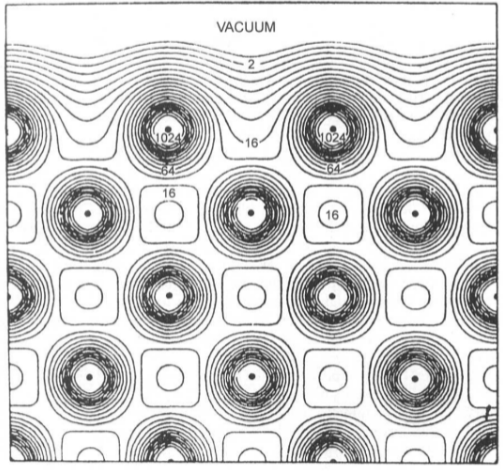
\includegraphics[width=\columnwidth]{images/surface.png}
    \label{fig:surface}
\end{figure}
\begin{itemize}
    \item Surface represent typcalliy \(15\)\r{A}
    \item At the surface, positiv periodic potential due to ions cores terminates
    \item Electrons will screen out at the surface resulting in  increased electron density
    \item At the surface, charge density is smeared out and less periodic compared to the interior ion cores(potential decrease)
    \item This smoothing of the surface charge is the compromise electrons strike when they lower both their potential and kinetic energies
    \item Band bending or new states happen at the surface
\end{itemize}
\begin{figure}[h]
    \centering
    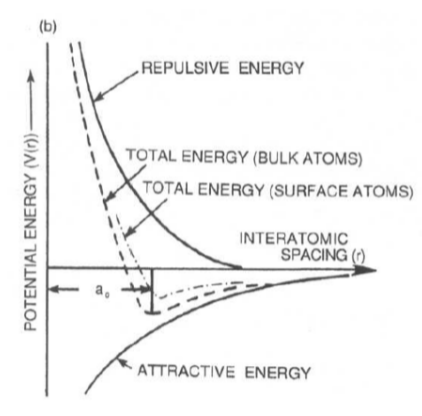
\includegraphics[width=\columnwidth]{images/atombond.png}
    \label{fig:atombond}
\end{figure}
\subsubsection{Adsorption on solid surface}
\begin{figure}[h]
    \centering
    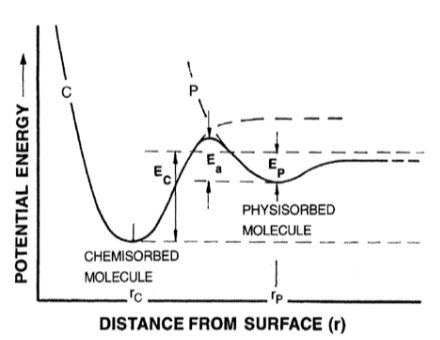
\includegraphics[width=\columnwidth]{images/surfacedistance.png}
    \label{fig:surfdist}
\end{figure}
\textbf{Surface adsorption: }Impinging atoms and molecules enter and interact within the transition region between gas phase \& Surface

Two kinds:
\begin{itemize}
    \item \textbf{Physisorption:} Van der waals force bond particel to the Surface
    \item \textbf{Chemisorption:} Particel changes identity through ionic or covalnet bonding with subtrate atoms
\end{itemize}

\subsection{Capillary theory of nucleation}
\begin{figure}[h]
    \centering
    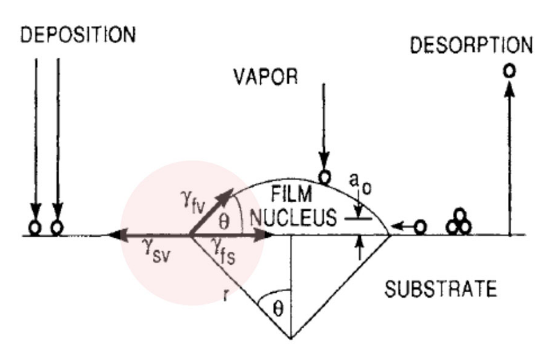
\includegraphics[width=0.7\columnwidth]{images/nucleation.png}
    \label{fig:nucleation}
\end{figure}
Film forming atoms or molecules in the vapor phase impinge on the substrate creating nuclei of mean dimension \(r\)

Free-energy change:
\[
\Delta G = a_3 r^3 \Delta G_v + a_1 r^2 \gamma_{fv} + a_2 r^2 \gamma_{fs} - a_2 r^2 \gamma_{sv}
\]
Mechanical equilibrium among horizontal components(Youngs equation):
\[
\gamma_{sv} = \gamma_{fs} + \gamma_{fv} \cos(\theta)\quad\text{or}\quad \cos(\theta) = (\gamma_{sv} -\gamma_{fs})/\gamma_{fv}
\]
Critical nucleus size \(r = r^*\):
\[
r^* = \frac{-2(a_1 \gamma_{fv}+a_2 \gamma_{fs} - a_2 \gamma_{sv})}{3 a_3 \Delta G_v}
\]
\subsection{Film growth modes}
Island growth:
\[
 \gamma_{sv} < \gamma_{fs} + \gamma_{fv}
\]
Layer growth:
\[
\gamma_{sv} \ge \gamma_{fs} + \gamma_{fv}
\]
\begin{figure}[!ht]
    \centering
    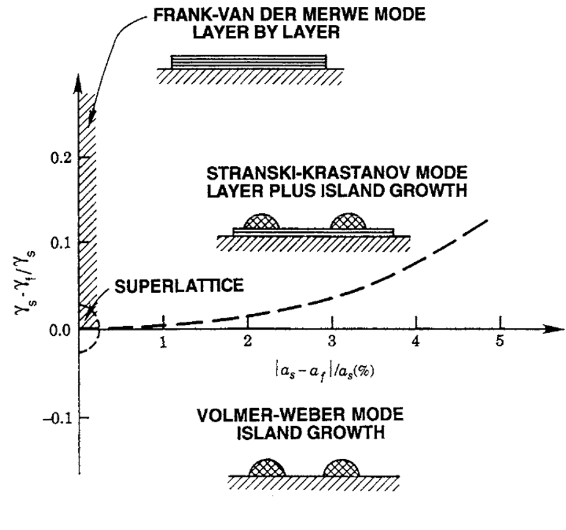
\includegraphics[width=\columnwidth]{images/layergrowth.png}
    \label{fig:layergrowth}
\end{figure}
\begin{figure}[!ht]
    \centering
    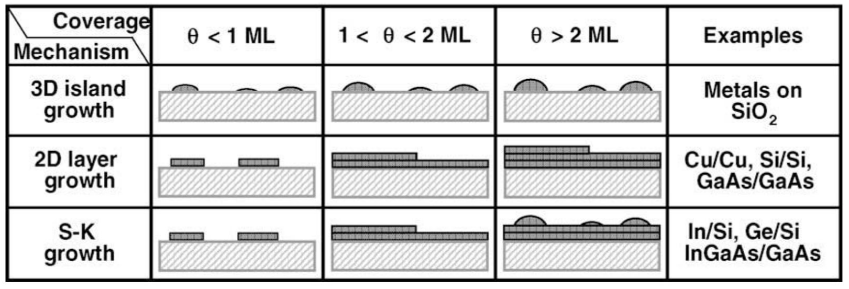
\includegraphics[width=\columnwidth]{images/growthmode2.png}
    \label{fig:growthmode2}
\end{figure}

\subsection{Dewetting}
\begin{figure}[h]
    \centering
    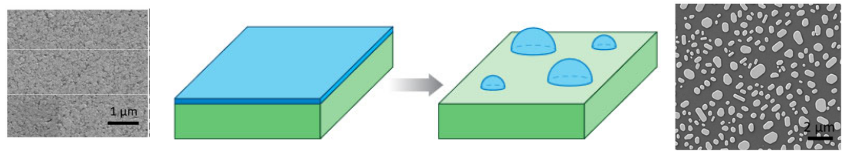
\includegraphics[width=\columnwidth]{images/dewetting.png}
    \label{fig:dewetting}
\end{figure}
During solid-state dewetting, thin films dewet to form isolated islands. This occures while the material remains in the solid state.
\begin{itemize}
    \item Thin films dewet or agglomerate to form arrays of islands when heated.
    \item This can happen when a films melting temperatures so that dewetting (agglomeration) occures while the film remains in the solid state.
    \item Driving force: minimization of the total energy of the free surfaces of the film and substrate, and of the film-substrate interface.
\end{itemize}

\subsection{Calculation of Surface energy}
OWRK-model:
\[
\sigma_{SL} = \sigma_{S} + \sigma_{L} - 2\sqrt{\sigma_S^d\sigma_L^d} - 2\sqrt{\sigma_S^p\sigma_L^p}
\]
With Youngs equation get linear equation \(y = mx + c\):
\[
\underbrace{\frac{\sigma_L (1+\cos(\Theta))}{2\sqrt{\sigma_L^d}}}_{y} 
= 
\underbrace{\sqrt{\sigma_S^p}}_{m}
\cdot
\underbrace{\frac{\sigma_L^p}{\sigma_L^d}}_{x} 
+ 
\underbrace{\sqrt{\sigma_s^d}}_{c}
\]
\(\sigma\) sometimes given as \(\gamma\)

\(S\): Solid

\(V\): Vapor

\(L\): Liquid

\section{Stress in thin film}
Film exerts bending moment on substrate plate which leads to curvature \((K = 1/R)\)
\begin{figure}[h]
    \centering
    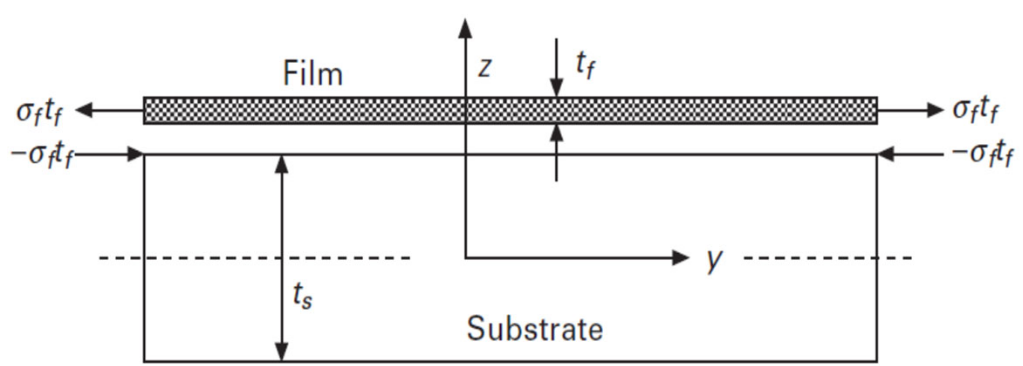
\includegraphics[width=\columnwidth]{images/stoney.png}
    \label{fig:stoney}
\end{figure}

\textbf{Stoney equation:}
\[
\sigma_f = \left(\frac{E_s}{1-v_s}\right)\frac{t^2_s}{6 t_f}\Delta \kappa
\]
Term \(\left(\frac{E_s}{1-v_s}\right)\) is called biaxial elastic modulus.

\(\kappa\): Curvature

Stoney equation is independent of film properties. Appliccable for thin film on a much thicker substrate.

\textbf{Methods for residual stress measurments:}
\begin{itemize}
    \item \textbf{Mechanical methods:} Substrate curvature vie laser deflection, bending of Focused Ion Beam(FIB) bi-metal beam
    \item XRD, Raman specrtoscopy 
\end{itemize}

Method comperison: Spatial (lateral \& depth), and spectral resolution

Stress types:
\begin{itemize}
    \item \textbf{Thermal:} Mismatch of thermal expansion coefficients
    \item \textbf{Intrinsic:} During Film growth
    \item \textbf{epitaxial(Misfit):} Lattice mismatch with substrate
\end{itemize}

\begin{figure}[h]
    \centering
    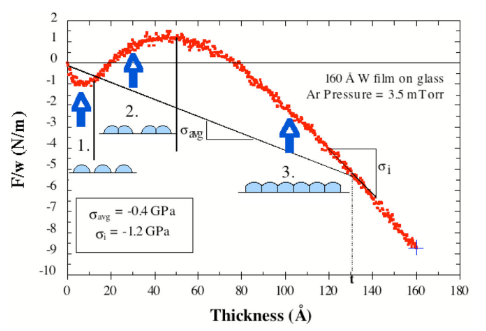
\includegraphics[width=\columnwidth]{images/insitu.png}
    \label{fig:insitu}
\end{figure}

\textbf{The stress dilemma:} intrinsic stress relaxes at high deposition T, thermal increases

\subsection{Adhesion of thin films}

Stress intensity at crack tip:
\[
K = 0.7 \sigma\sqrt{h}
\]

Energy release rate if interface crack propagates:
\[
G = 0.5 \frac{1-v^2}{E}\sigma^2 h
\]

\textbf{Strategies against bad film adhesion - glue layers:} It is common to first deposit a fed hundered angstroms of an intermediate oxygen-active metal to serve as the \textit{glue} between the film and substrate.

Scratch Testing:
\begin{itemize}
    \item Draw diamond tip across surface with increasing normal load until a critical event occures
    \item Film will debond(form buckle) or fracture(form through thickness cracks)
\end{itemize}

\subsection{Hard Coatings}
Hard materials: mixed bonds(covalent + metallic + ionic)
Three groups are distinguished based on chemical bonding:
\begin{itemize}
    \item \textbf{metallic hard materials}(covalent + metallic)
    \subitem +: adhesion, toughness ductility, high elastic modulus
    \item \textbf{ionic hard materials}(covalent + ionic)
    \subitem +: hardness, thermodynamic stability, \\chemical inertness
    \subitem -: very brittle
    \item \textbf{covalent hard materials}(covalent + ionic)
    \subitem +: hardest materials(Diamond), strength, high temperature strength, low thermal expension coefficant
    \subitem -: not adapted to metallic substrate at HT
\end{itemize}

The \textbf{intrinsic hardness }related to:
\begin{itemize}
    \item high binding energy (bond strength)
    \item short interatomic distance (small bond lenght)
    \item high degree of directional covalent bonds(ionicity and metallicity decrease hardness)
    \item high number of valence electrons per atom
    \item high number of bonds per unit volume
\end{itemize}